\chapter[Multitudes of Objects: First Implementation and Case Study for Java]{\texorpdfstring{%
Multitudes of Objects\\{\Large{}First Implementation and Case Study for Java}}{%
Concurrent Evaluation of Reference Attribute Grammars}}
\label{ch:multiplicities}
\paperRemark{\paperIIref}

%\affiliation{fernuni}{Lehrgebiet Programmiersysteme, Fernuniversität in Hagen, Germany}
%\affiliation{lu}{Lund University, Sweden}

{
% XeLaTeX stuff
%\setmonofont{Courier}

\makeatletter
\def\uwavered{\bgroup \markoverwith{\lower3.5\p@\hbox{\sixly \textcolor{red}{\char58}}}\ULon}
\font\sixly=lasy6 % does not re-load if already loaded, so no memory problem.
\makeatother

%\DeclareSortingScheme{customsort}{
%  \sort{\field{key}}
%}
%
%\AtEveryBibitem{\clearfield{url}}% remove doi urls

\makeatletter
\newenvironment{CenteredBox}{%
\begin{Sbox}}{%
\end{Sbox}\centerline{\parbox{\wd\@Sbox}{\TheSbox}}}%
\makeatother

\def\something{\ldots}

%\renewcommand{\ttdefault}{pcr}
\lstset{
  language=Java,%
  showstringspaces=false,
  %emph={abstract},%
  %emphstyle={\color{black}\bfseries\underbar},%
  morekeywords={any,option},%
  basicstyle=\ttfamily,
  %columns=flexible,%
  mathescape=true%
  %literate=
    %{*(}{\color{blue}}1
    %{)*}{\normalcolor}1
}

%\newcommand{\g}[1]{{\setlength{\fboxsep}{0pt}\colorbox{lightgray}{#1}}}
\newcommand{\g}[1]{\adjustbox{bgcolor=lightgray}{\strut{}#1}}
\newcommand{\f}[1]{\textbf{#1}}

\usetikzlibrary{matrix,shapes.multipart,trees,calc,arrows}

\renewcommand*{\sectionautorefname}{Section}
\renewcommand*{\subsectionautorefname}{Section}
\renewcommand*{\subsubsectionautorefname}{Section}

\section*{Abstract}

In object-oriented programs, the relationship of an object to many
objects is usually implemented using indirection through a collection. This
is in contrast to a relationship to one object, which is usually implemented
directly. However, using collections for relationships to many objects does
not only mean that accessing the related objects always requires accessing
the collection first, it also presents a lurking maintenance problem that
manifests itself when a relationship needs to be changed from to-one to
to-many or vice versa. Continuing our prior work on fixing this problem, we
show how we have extended the Java 7 programming language with
multiplicities, that is, with expressions that evaluate to a number of
objects \emph{not} wrapped in a container, and report on the experience
we have gathered using these multiplicities in a case study.

\begin{flushright}
  \emph{ein Vieles, welches kein Eines ist}\\
  (\emph{a multitude which is not a one})\\
--- inspired by Georg Cantor's conception of a set as ``jedes Viele, welches
sich als Eines denken l{\"a}{\ss}t'', i.e., any multitude which can be thought of as a
one
\end{flushright}

\section{Introduction}

\noindent Just like English grammar distinguishes singular and plural,
object-oriented programming languages distinguish one object and many
objects. However, unlike with English utterances, for which the syntactic
difference between the singular and the plural of a noun phrase is usually
small, the difference between program fragments dealing with one object and
dealing with many objects is often substantial. For instance, while the
English utterances ``I go to work'' and ``we go to work'' differ only
in the pronoun used, in an object-oriented program, the difference would be
that between \inline{i.goto(work)} and \inline{for (each : we) each.goto(work)},
which is cumbersome not only by comparison. The problem, here, is that in
object-oriented programming, the multitude denoted by \inline{we} is reified
as a one (usually a collection object), and this one has different
properties (responds to a different protocol) than the objects it comprises.
In particular, the object denoted by \inline{we} cannot go to work.

\begin{figure}
  \resizebox{\textwidth}{!}{%
  \begin{tikzpicture}[
      arrow/.style={
        ->,
        line width=1pt
      },
      divider/.style={
        draw=blue!40
      },
      heading/.style={
        fill=black!10
      }
    ]
    \node[draw] (c1) {\sffamily{Customer}};
    \node[draw,xshift=1.3cm,anchor=west] at(c1.east) (a1) {\sffamily{Account}};
    \draw[arrow] (c1.east) -> node[above,midway] {\footnotesize{\sffamily{account}}} node[below,near end] {\footnotesize{0..1}} (a1.west);

    \node[heading,anchor=south,yshift=5mm] (one) at($ (c1.north west) !.5! (a1.north east) $) {to-one relationship};

    \node[heading,anchor=east,xshift=-4mm] at(c1.west) {modelling};

    \node[anchor=west,draw,xshift=1cm] (c2) at(a1.east) {\sffamily{Customer}};
    \node[draw,xshift=1.3cm,anchor=west] at(c2.east) (a2) {\sffamily{Account}};
    \draw[arrow] (c2.east) -> node[above,midway] {\footnotesize{\sffamily{account}}} node[below,near end] {\footnotesize{0..*}} (a2.west);

    \node[heading,anchor=south,yshift=5mm] at($ (c2.north west) !.5! (a2.north east) $) {to-many relationship};

    \node[anchor=north,yshift=-1cm,draw, rectangle split, rectangle split parts=2] (c3) at(c1.south) {
      \nodepart{one}\sffamily{Customer}
      \nodepart{two}\sffamily{account}
    };
    \node[draw,xshift=1.3cm,anchor=west] (a3) at(c3.one east) {\sffamily{Account}};
    \draw[arrow] (c3.two east) -> node[below,near end] {\footnotesize{0..1}} (a3.west);

    \node[heading,anchor=east,xshift=-4mm] (impl) at(c3.west) {programming};

    \node[anchor=north west,xshift=1cm,draw, rectangle split, rectangle split parts=2] (c4) at(a3.north east) {
      \nodepart{one}\sffamily{Customer}
      \nodepart{two}\sffamily{accounts}
    };
    \node[draw,xshift=1.3cm,anchor=west] at(c4.one east) (ac4) {\sffamily{Collection}};
    \node[draw,yshift=-8mm] at(ac4.south) (a4) {\sffamily{Account}};

    \draw[arrow] (c4.two east) -> node[below,near end] {\footnotesize{0..1}} (ac4.west);
    \draw[arrow] (ac4) -> (a4);
    \node[xshift=-5pt,yshift=5pt] at (a4.north east) {\footnotesize{0..*}};

    \coordinate[xshift=-5mm] (vcenter) at(c2.west);
    \coordinate[yshift=5mm] (hcenter) at(c3.north);
    \coordinate (p1) at(one.north -| vcenter);
    \coordinate (p2) at(a4.south -| vcenter);
    \coordinate (p3) at(impl.west |- hcenter);
    \coordinate (p4) at(ac4.east |- hcenter);
    \draw[divider] (p1) -- (p2);
    \draw[divider] (p3) -- (p4);

  \end{tikzpicture}
  }%resizebox
  \caption{Relationships to one and to many objects in
object-oriented modelling and programming languages: differences}
  \label{figure1}
\end{figure}

Similar to the English language, relational and object-oriented modelling
languages make only a small distinction between singular and plural or, more
specifically, between one object being associated with one other, or any
number of other objects \cite{ref8, ref9, ref10, ref28, ref36}. In these languages,
\emph{multiplicity}, also known as \emph{cardinality}, constrains
the number of times an object, or entity, may occur in a relationship or
association. Hence, a change from singular to plural (or vice versa)
requires little more than a corresponding change in multiplicity, as the top
half of \autoref{figure1} suggests. By contrast, in object-oriented programming
languages multiplicities are commonly coded in the declared type of a
variable (which is the type of the related object if it is only one, or the
type of a sequence, stream, or collection object if there are more). Here, a
change of multiplicity may require a major redesign of the program, as the
bottom half of \autoref{figure1} suggests (several more untoward consequences of such
a change will be presented below).

In previous work \cite{ref37}, we advocated the introduction of
\emph{multiplicities} as annotations of expressions indicating whether
an expression is singular or plural, i.e., whether it is expected to
evaluate to at most one object, or to any number of objects~(not reified).
This is to grant the programmer a more uniform treatment of relationships to
one object and relationships to many objects in object-oriented programs. In
this paper, we present an implementation of our ideas as an extension of the
Java programming language using the JastAddJ extensible Java compiler \cite{ref13},
and report on a case study we have conducted.

The remainder of this paper is organized as follows. To motivate our work,
we present in \autoref{section2} the peculiarities we observe when implementing
multitudes of objects using collections. In \autoref{section3}, we briefly describe
how enhancing object-oriented programming with multiplicities can generally
alleviate the associated problems, with \autoref{section4} specializing our proposal
for Java. \autoref{section5} describes our implementation of multiplicities as an
extension of the JastAddJ compiler for Java 7. In \autoref{section6}, we present
qualitative and quantitative findings from a case study extending JUnit with
multiplicities. Notes on related and future work conclude.

\section[Using Collections for Representing Multitudes of Objects]{\texorpdfstring{%
\raggedright Using Collections for Representing Multitudes of Objects}{%
Using Collections for Representing Multitudes of Objects}}
\label{section2}

\noindent Undoubtedly, collections are among the most useful abstractions in
object-oriented programming: they not only liberate the programmer from
manually implementing multitudes of objects as (static) arrays or dynamic
data structures (such as linked lists or trees), they also offer a uniform
protocol for bulk processing of these object using internal iterators
(\inline{foreach}, \inline{select}, \inline{collect}, etc.). And yet, the use of
collections for representing many (rather than one) objects comes with a
number of peculiarities which make dealing with multitudes of objects very
different from dealing with single objects.

\subsection{Multiplicity Determines Type}
\label{section2.1}

\noindent In a program in which every customer can have only a single
account, we may see code like

\begin{lstlisting}
Account account;
account = new Account();
account.check();
\end{lstlisting}

\noindent If however a customer can have several accounts, adjustment of
just the declaration to reflect this leads to an ill-typed program (faulty
expressions underlined):

\begin{lstlisting}
Set<Account> accounts;
$\uwavered{\texttt{accounts = \textbf{new} Account();}}$
$\uwavered{\texttt{accounts.check();}}$
\end{lstlisting}

\noindent Both errors result from the fact that \inline{accounts} (with a
plural ``s'' appended to express that there can be more than one) now has
type \inline{Set<Account>}, reflecting the changed multiplicity. However, intuitively,
what is expressed by the ill-typed program is rather clear: initialize
\inline{accounts} to hold just one account, and then check all accounts (which
happens to be only one here). To translate this to standard Java, we would
have to write

\begin{lstlisting}
Set<Account> accounts = new HashSet<>();
accounts.add(new Account());
for (Account account : accounts) account.check();
\end{lstlisting}

\noindent which means quite a change to the original program.

\subsection{Multiplicity Determines Meaning of \texttt{null}}
\label{section2.2}

\noindent When a variable represents an optional relationship to one object,
the value \inline{null} usually means that there is no relationship (but may
also mean failure to initialize):

\begin{lstlisting}
if (account != null) print(account);
else print("no account");
\end{lstlisting}

\noindent For a relationship to many accounts, relating to no account is
usually represented using an empty collection:

\vbox{
\begin{lstlisting}
if (accounts != null)
  if (! accounts.isEmpty())
    for (Account account : accounts) account.print();
  else print("no account");
else throw new Error("accounts not initialized");
\end{lstlisting}
}

\noindent Here, the value \inline{null} means failure to
initialize. Note that having \inline{null} as an element of a collection makes
no sense if the collection is to represent a relationship.

\subsection{Multiplicity Determines Subtyping Conditions}
\label{section2.3}

\noindent If \inline{SavingsAccount} is a subtype of \inline{Account}, writing

\begin{lstlisting}
SavingsAccount saving = new SavingsAccount();
Account account = saving;
\end{lstlisting}

\noindent is type-correct. However, when we change to many accounts, the
analogue

\begin{lstlisting}
Set<SavingsAccount> savings = new HashSet<>();
Set<Account> accounts = savings;
\end{lstlisting}

\noindent is ill-typed. Instead, we would have to write something like

\begin{lstlisting}
Set<? extends Account> accounts = savings;
\end{lstlisting}

\noindent \cite{ref24} which does however preclude write access to the set through
the variable \inline{accounts}, greatly limiting its use (especially when
considering that the singular \inline{account} can be used freely).

\subsection{Multiplicity Determines Encapsulation Strategy}
\label{section2.4}

\noindent It is considered good practice in object-oriented programming that
the fields of an object are encapsulated and, if necessary, made accessible
for clients using setter and getter methods. For collection-valued fields,
however, this is different \cite{ref16}: they are to be updated using \inline{add...($\something$)} and
\inline{remove...($\something$)} methods offered by the encapsulating object (where the ellipses
are replaced by the field's name), and if the collection as a whole is
to be retrieved, the getter should return a copy or an immutable wrapper
\cite{ref16}. This is so because the collection is considered a representation
object which clients should not be able to manipulate directly and of which
they should possess no aliases \cite{ref25}. This brings us directly to the next
point.

\subsection{Multiplicity Determines Availability of Relationship Aliasing}
\label{section2.5}

\noindent While assigning an object to a variable with reference semantics
always means creating an alias for the object, the semantics differ when the
variables are uniformly viewed as implementing relationships to objects, as
the following example demonstrates:

\begin{lstlisting}
Account backup = account;
account = null;
if (mistaken) account = backup;
\end{lstlisting}

\noindent Here, \inline{backup} is an alias for the to-one relationship
implemented by \inline{account}. This is different for

\begin{lstlisting}
Collection<Account> backups = accounts;
accounts.clear();
if (mistaken) accounts = backups;
\end{lstlisting}

\noindent where \inline{backups} is an alias for the collection denoted, and
not for the to-many relationship that is logically established, by
\inline{accounts}. Surely, the problem can be solved by keeping a copy of the
collection as backup, but copying is not needed for the to-one case.

\subsection{Multiplicity Determines Call Semantics}
\label{section2.6}

\noindent Continuing the previous example, it may seem awkward that the
method

\begin{lstlisting}
void clear(Collection<Account> accounts) {
  accounts.clear();
}
\end{lstlisting}

\noindent performs as intended (i.e., sets the relationship represented by
an actual parameter to ``no accounts''), while the analogous method for
the to-one case

\begin{lstlisting}
void clear(Account account) {
  account = null;
}
\end{lstlisting}

\noindent has no effect on actual parameters. While this may look like a
newbie's mistake to the seasoned programmer, it is still indicative of
a conceptual chasm, which culminates in the fact that in Java, it is
impossible to implement

\begin{lstlisting}
void swap(Object o1, Object o2)
\end{lstlisting}

\noindent with the suggested semantics, while implementing

\begin{lstlisting}
void sort(ArrayList<Object> os)
\end{lstlisting}

\noindent is not a problem. Note that escaping to call-by-reference for
\inline{swap($\something$, $\something$)} does not bridge the chasm --- not having to do so for collections
is just another peculiarity of using them for representing multitudes of
objects.

\subsection{Multiplicity Determines Meaning of the \texttt{final} Modifier}
\label{section2.7}

\noindent When a variable is declared as \inline{final}, it means that its
value cannot be changed after its initialization. For a variable
representing a relationship to a single object this means that the owner of
the variable is stuck with the related object for its whole lifetime. For a
variable representing a relationship to many objects implemented using a
collection, \inline{final} means that the holder of the relationship is stuck
with the collection --- its elements, and thus the conceptually related
objects, may change freely:

\begin{lstlisting}
final Account forLife = new Account();
forLife = null; // compile error

final Set<Account> allForLife = Arrays.asSet(forLife);
allForLife.clear(); // no problem
\end{lstlisting}

\section{Programming with Multiplicities}
\label{section3}

\noindent The core idea of object-oriented programming with multiplicities
as put forward in \cite{ref37} is that expressions may evaluate directly to any
number, or \emph{a multitude}, of objects. This is in
contrast to standard object-oriented programming, in which every expression
evaluates to either one object or to \inline{null} and in which multitudes of
objects are reified using special container objects (collections, sequences,
iterators, etc.). Note that, since multitudes are not reified in our
approach, they are always flat, i.e., there is no multitude of multitudes
(though it is possible to create a multitude of collections).

% removed colon after "Terminological Note"
\paragraph{Terminological Note} We use ``multitude of objects'' to denote many objects;
the term is to be distinguished from ``collection of objects'' or
``set of objects'', which each denote an entity in its own right. Note that for
this reason it makes no sense to speak of ``the elements'' or ``the
members of a multitude'', or even of ``the objects of a multitude'' (since
the objects of the multitude \emph{are} the multitude) --- if we want
to refer to one of many, we say just that, or ``one object among
a multitude''.

\subsection{Dynamic and Static Multiplicity}
\label{section3.1}

\noindent With expressions evaluating to any number of objects, the
\emph{dynamic multiplicity} of an expression is defined as the number
of objects it evaluates to. In the general case, the dynamic multiplicity of
an expression can only be determined at runtime. Therefore, we complement
dynamic multiplicity with \emph{static multiplicity}, which can be
declared and inferred at compile-time. In the following, the term
multiplicity refers to static multiplicity unless stated otherwise.

While dynamic multiplicities are cardinals, we distinguish mainly two
(symbolic) static multiplicities, which we call \emph{option} and
\emph{any}. \emph{Option} stands for no or one ob\-ject, while
\emph{any} stands for any number of objects. Other static
multiplicities are also conceivable (in particular, multiplicity \emph{one}, for
precisely one, will be useful; see below); however, since our focus here is
on eliminating as much as possible the differences between relating to zero or one and to any number of objects, \emph{option} and \emph{any} suffice.

\subsection{Separation of Multiplicity and Type}
\label{section3.2}

\noindent As long as multitudes of objects are reified, the multiplicity of
an expression (i.e., whether it evaluates to one or many objects) is coded
in its type: for multiplicity \emph{any}, this type is a collection
type (commonly parameterized with the member type, i.e., the type of the
elements of the collection), whereas for multiplicity \emph{option},
the type is the type of the optional object (see \autoref{section2.1}). Object-oriented
programming with multiplicities as put forward in \cite{ref37} separates
multiplicity from type in the declaration of variables and methods: for
instance, it allows one to write

\begin{lstlisting}
any Account accounts;
\end{lstlisting}

\noindent instead of

\begin{lstlisting}
Collection<Account> accounts;
\end{lstlisting}

\noindent for declaring that \inline{accounts} can hold any number of
\inline{Account} objects (note that it cannot hold a collection!), whereas

\begin{lstlisting}
option Account account;
\end{lstlisting}

\noindent which differs only in the multiplicity, is roughly equivalent to

\begin{lstlisting}
Account account;
\end{lstlisting}

\noindent meaning that \inline{account} can hold either no or one account
(see \autoref{section3.4} for the important difference).  Note that using
multiplicities, both \inline{account} and \inline{accounts} have the same type
\inline{Account}; they differ only in their declared multiplicities.

\subsection{Assignment Compatibility}
\label{section3.3}

\noindent While the types of \inline{account} and \inline{accounts} are the same
and, therefore, do not oppose their mutual assignment compatibility, their
multiplicities differ --- since \emph{option} is subsumed
by \emph{any}, \inline{account} can be assigned to \inline{accounts}, and

\begin{lstlisting}
any Account accounts = new Account();
\end{lstlisting}

\noindent is a legal assignment (cf.~\autoref{section2.1}). An assignment from
\emph{any} to \emph{option} is illegal, however; here, a
multiplicity downcast (from \emph{any} to \emph{option}) as in

\begin{lstlisting}
account = (option) accounts;
\end{lstlisting}

\noindent is required, but may fail at runtime (namely when \inline{accounts}
holds more than one object).

For variables with multiplicity \emph{any}, assignment is
complemented with adding to (\inline{+=}) and subtracting from (\inline{-=})
a multitude of objects, where the right-hand side of the update operations
can have multiplicity \emph{any} or \emph{option}.

   \inline{null} remains assignment compatible with every reference type;
also, it is assignment compatible with both multiplicity \emph{option}
and \emph{any} (and means ``related to no object'' in both cases;
cf.~\autoref{section2.2}).

\subsection{Member Access}
\label{section3.4}

\noindent That \inline{account} and \inline{accounts} have the same type means
that they respond to the same protocol, i.e., that the same set of methods
can be invoked and the same set of fields can be accessed on them. For
instance, if class \inline{Account} defines a method \inline{check()}, both
\inline{account.check()} and \inline{accounts.check()} are well-typed; the
latter simply means that \inline{check()} is separately invoked on all objects
\inline{accounts} holds. If \inline{Account} declares an \emph{option} field \inline{bank},
\inline{accounts.bank} returns a multitude of bank objects, namely the
banks each account among the multitude of accounts held by \inline{accounts}
is related to. Note that if \inline{accounts} holds no object, or no account
referred to by \inline{accounts} has a bank associated with it,
\inline{accounts.bank} will evaluate to no object. Since \emph{option} is
subsumed by \emph{any}, \inline{account.bank} will also evaluate to no object
if \inline{account} does not hold an account; note in particular that no null
pointer exceptions can arise from dereferencing expressions whose
multiplicity is \emph{option} or \emph{any}.\footnote{For the relationship of the multiplicity \emph{option}
with the type \inline{Option} of some functional programming languages
(including Scala), see the related work in \autoref{section7}}

\subsection{Aliasing}
\label{section3.5}

\noindent In object-oriented programming with multiplicities, multitudes of
objects are not reified, so multitudes cannot be aliased. This retires the
problems noted in Sections~\ref{section2.3}--\ref{section2.6}. In particular,

\begin{lstlisting}
any SavingsAccount savings;
any Account accounts = savings;
\end{lstlisting}

\noindent does not cause a covariance problem, since the assignment does not
create an alias for a container, but instead assigns \inline{accounts} the
same multitude of objects that \inline{savings} refers to (by copying pointers
just like in the \emph{option} case). It follows that

\begin{lstlisting}
accounts += new Account();
\end{lstlisting}

\noindent does not also add an account to \inline{savings} (cf.~\autoref{section2.3}).
Likewise, returning \inline{accounts} as in

\begin{lstlisting}
any Account getAccounts() { return accounts; }
\end{lstlisting}

\noindent does not expose representation to clients (there is no
representation object representing the multitude held by \inline{accounts})
and, in particular,

\begin{lstlisting}
any Account temp = getAccounts();
temp += new Account();
\end{lstlisting}

\noindent does not update the field \inline{accounts} returned by the getter
(\autoref{section2.4}). Similarly, after the assignment

\begin{lstlisting}
any Account backups = accounts;
\end{lstlisting}

\noindent (\autoref{section2.5}), clearing \inline{accounts} (by assigning it \inline{null};
cf.~\autoref{section3.3}) does not also clear \inline{backups}, which is therefore still
available for restoration. Also, passing a variable into the method
\inline{clear($\something$)} of \autoref{section2.6}, now defined as

\vbox{
\begin{lstlisting}
void clear(any Account accounts) {
  accounts = null;
}
\end{lstlisting}
}

\noindent does not affect the number of objects that this variable holds,
thereby unifying the behaviour for one and many objects. Lastly, the fact
that multitudes of objects are not reified unifies the meaning of the
\inline{final} modifier (\autoref{section2.7}), which now pertains to variables holding
single object and multitudes of objects alike.

\subsection{When to and When Not to Use Multiplicities}
\label{section3.6}

Our motivation of introducing multiplicities to object-oriented programming
is to allow the programmer

\begin{itemize}
  \item the implementation of relationships (or, more precisely, directed
    associations \cite{ref28}) to many objects in a more direct way, and further
  \item the implementation of relationships to one and to many objects in as
    much the same way as possible.
\end{itemize}

\noindent This raises the question of what is a relationship, or when
multiplicities are to be used.

Experience teaches that programmers will use a construct wherever they
deem its use advantageous, so we attempt no dogmatism here. We still make
one exception, though: value types, like \inline{int}, \inline{float},
\inline{boolean}~(including their wrapper types), or \inline{String} (whose
instances are usually immutable) cannot be the target of a relationship
(note that they cannot act as entity types in the entity-relationship model
\cite{ref8}) and hence cannot be used in combination with \emph{option} or
\emph{any} multiplicity annotations. While there are conceptual
justifications for this (e.g., people do not relate to their age, an integer
value), the main technical reason is that this saves us from defining
special semantics for operations on value types (such as \inline{+}) for operands
with \emph{option} or \emph{any} multiplicity (which both include
``no object'' as a possible value), and also from introducing a ternary logic
for handling the case that a boolean expression used in a conditional
evaluates to no object. For instance, for a variable declared as
\inline{option boolean error}, it is unclear what \inline{if (error) ...} means
if \inline{error} has dynamic multiplicity 0. For the same reason, we must
exclude that value-typed members are accessed via receiver expressions with
\emph{option} or \emph{any} multiplicity, since this can likewise
result in dynamic multiplicity 0 (namely when the receiver evaluates to
``no object'').

\section{Multiplicities for Java}
\label{section4}

\noindent While the idea of object-oriented programming with multiplicities
as presented in the previous section is language-independent, its adoption
in any concrete language invariably requires an individualized integration
with existing language constructs. In the following, we present our
extension of Java 7 with multiplicities, whose design was driven by our
objective to allow a smooth transition between Java programming without and
Java programming with multiplicities. \autoref{figure2} has the extended syntax;
\autoref{figure3} shows some sample code using it.

\begin{figure}[h]
  \begin{CenteredBox}
\begin{lstlisting}[basicstyle=\ttfamily\small]
Modifier ::= ...
 | MultiplicityAnnotation;

MultiplicityAnnotation ::=
   "@any" "(" ReferenceType ")"
 | "@any"
 | "@option"
 | "@bare";

Primary ::=
 | "[[" UnaryExpressionNotPlusMinus "]]"
 | "|[" UnaryExpressionNotPlusMinus "]|";

CastExpression ::= ...
 | MultiplicityCastExpr;

MultiplicityCastExpr ::=
   "(" MultiplicityAnnotation ")" UnaryExpression
 | "(" MultiplicityAnnotation TypeName ")"
   UnaryExpression;
\end{lstlisting}
  \end{CenteredBox}
\caption{Extension of concrete syntax.}
\label{figure2}
\end{figure}

\begin{lrbox}{\lstboxleft}
\begin{lstlisting}[basicstyle=\ttfamily\footnotesize]
class Subject implements Observable {
  $\g{Set<}$Observer$\g{>}$ obs $\g{= new HashSet<>()}$;

  public void addObserver(Observer o) {
    $\g{if (o == null)}$
      $\g{throw new NullPointerException();}$
    obs$\g{.add(}$o$\g{)}$;
  }

  public void deleteObserver(Observer o) {
    obs.$\g{remove(}$o$\g{)}$;
  }

  public void notifyObservers(Object arg) {
    $\g{for (Observer o :}$ obs$\g{)}$
      $\g{o}$.update(this, arg);
  }

  public void deleteObservers() {
    obs$\g{.clear()}$;
  }

  public int countObservers() {
    return obs$\g{.size()}$;
  }
}
\end{lstlisting}%
\end{lrbox}

\begin{lrbox}{\lstboxright}
\begin{lstlisting}[basicstyle=\ttfamily\footnotesize]
class Subject implements Observable {
  $\g{@any(}$HashSet$\g{)}$ Observer obs;

  public void addObserver($\g{@option}$ Observer o) {


    obs $\g{+=}$ o;
  }

  public void deleteObserver($\g{@option}$ Observer o) {
    obs $\g{-=}$ o;
  }

  public void notifyObservers(Object arg) {

    obs.update(this, arg);
  }

  public void deleteObservers() {
    obs $\g{= null}$;
  }

  public int countObservers() {
    return $\g{|[}$obs$\g{]|}$;
  }
}
\end{lstlisting}%
\end{lrbox}

\begin{figure}[b!]
\begin{CenteredBox}
  \begin{tabular}{cc}
    original (without using multiplicities) & using multiplicities \\
    \hline
    \scalebox{0.8}{\usebox{\lstboxleft}}&%
    \scalebox{0.8}{\usebox{\lstboxright}}\\
  \end{tabular}
\end{CenteredBox}
  \caption{Example of implementing class \inline{Subject} of the Observer
    Pattern, with and without using multiplicities (differences highlighted)}
  \label{figure3}
\end{figure}

\subsection{Multiplicity Annotations}
\label{section4.1}

\noindent For compatibility with existing Java code, we implemented four
static multiplicities:

\begin{itemize}
  \item \emph{none}, the multiplicity of \inline{null} (representing no object);
  \item \emph{bare}, the default multiplicity (and, in particular, the
    multiplicity of all standard, or legacy, declarations);
  \item \emph{option}, the multiplicity of entities and expressions
    representing relationships to no or to one object; and
  \item \emph{any}, the multiplicity of entities and expressions representing
    relationships to any number of objects.
\end{itemize}

\noindent Multiplicities determine assignment compatibility according to the
order

\begin{equation*}
  none < bare < option < any
\end{equation*}

\noindent i.e., every multiplicity is assignment compatible with itself and
all greater ones.

\paragraph{Hidden Collections} To give the programmer control over the nature of
multitudes, and also for interfacing with legacy Java code that uses
collections (see below), \emph{any} multiplicities may be parameterized
with a collection type \emph{C} whose definition has a single type
parameter (e.g., \inline{List<E>}). This type will be used to instantiate a
\emph{hidden collection} holding the multitude of objects. To
acknowledge the widespread use of abstract collection types in Java
programs, \emph{C} may be an abstract class or an interface.

\paragraph{Syntactic Integration} The multiplicity \emph{none} does not occur in
program texts; the other multiplicities appear as annotations \inline{@bare},
\inline{@option}, and \inline{@any}, respectively (see~\autoref{figure2}). Since
\emph{bare} is the default multiplicity, it occurs only in multiplicity
downcasts from \emph{option} or \emph{any} to \emph{bare}
(see below).

\subsection{Declarations}
\label{section4.2}

\noindent The multiplicity annotations \inline{@option} and \inline{@any} may
appear (in the position of modifiers; cf. \autoref{figure2}) in all declarations of
reference-typed entities, except where the type is a wrapper type (such as
\inline{Boolean}) or \inline{String} (see \autoref{section3.6} for the reasons). If an
entity is annotated with \inline{@any(C)} and \inline{C} is a concrete
collection class, the compiler uses \inline{C} as the class of the hidden
collection that holds the multitude of objects the annotated entity denotes;
if \inline{C} is abstract or not provided, the compiler automatically picks a
suitable concrete class (note that the single type parameter of \inline{C} is
instantiated with the type of the declaration). Thus, multitudes of objects
\emph{are} implemented using collections; however, this implementation
is strictly under the hood and, in particular, these collections cannot be
accessed from the program as objects (they cannot be aliased). Entities
annotated with \inline{@option} are not implemented using collections;
however, the compiler gives their value \inline{null} a special meaning (see
below).

\paragraph{Final Declarations} A declaration \inline{final @option T v} means that,
after its initialization, the value of \inline{v} cannot change (i.e.,
\inline{v} always refers to the same object). That \inline{v} is not assigned
new values after initialization is ensured (by the compiler) as usual. A
declaration \inline{final @any T v} likewise means that \inline{v} cannot be
updated after its initialization (i.e., it always refers to the same
objects), where updating includes assignment (\inline{=}), adding objects (\inline{+=}), and
removing objects (\inline{-=}); this is ensured by the very same means. Hence,
no immutable collections are required to express the immutability of a
multitude.

\subsection{Interfacing with Collections: Wrapping and Unwrapping}
\label{section4.3}

\noindent To interface multiplicity \emph{any} with code that uses
(bare) collections for representing multitudes of objects, we must be able
to wrap a multitude in a collection object, and to unwrap it from a
collection object. We use double square brackets (``\inline{[[$\something$]]}'') for both purposes
(see \autoref{figure2}). If the argument expression has static multiplicity
\emph{any(C)}, the result is a (fresh) collection of type
\emph{C} holding the objects the expression evaluates to; if it has
multiplicity \emph{option}, the result is a new instance of class
\inline{ArrayList} which either holds the object the expression evaluates to,
or is empty if it evaluates to \inline{null}. We call this
\emph{wrapping}. If the argument expression has static multiplicity
\emph{bare} and is a collection, the result is the multitude of objects
that the collection holds (which is internally represented using a fresh
collection of the same type). We call this \emph{unwrapping}.
Unwrapping is particularly useful for initializing final variables with
multiplicity \emph{any}:

\begin{lstlisting}
final @any Account accounts =
  [[Arrays.asList(new Account(), new Account())]];
\end{lstlisting}

\noindent The expression \inline{[[null]]} is not allowed.

\subsection{Number of Objects}
\label{section4.4}

\noindent The dynamic multiplicity, or the number of objects an expression
evaluates to, is computed using ``\inline{|[$\something$]|}'' (see \autoref{figure2}). In case the argument
expression has multiplicity \emph{any}, it returns the size of the
underlying collection; if the expression has multiplicity
\emph{option}, it returns 0 if it evaluates to \inline{null}, and 1 else.

\subsection{Casts}
\label{section4.5}

As for types, multiplicity upcasts (e.g., from \emph{option} to
\emph{any}) are always safe and therefore may remain implicit.
Multiplicity downcasts from \emph{any} to \emph{option} or
\emph{bare}, however, may fail, namely when the \emph{any}
expression being cast evaluates to more than one object. Therefore, the
compiler inserts a runtime multiplicity check for all such casts which, upon
failure, throws a multiplicity cast exception. Casts from \emph{option}
to \emph{bare} are also always safe; since unlike for
\emph{option} receivers, accessing members on \emph{bare}
receivers can lead to null pointer exceptions, we will require explicit
downcasts from \emph{option} to \emph{bare} (see below for
examples of where this is needed).

\subsection{Expressions}
\label{section4.6}

\noindent With new syntax given meaning as above, we now turn to the impact
multiplicities have on standard Java expressions.

\paragraph{Update} Assignment (\inline{=}) makes the variable on the left-hand side refer to
the objects the right-hand side refers to. Given the arbitrariness of the
definition of ``identity of multitudes of objects'' for multiplicity
\emph{any} (see below), we defined assignment pragmatically: the hidden
collection holding the multitude of the left-hand side is first emptied
(cleared), and then all objects of the hidden collection representing the
right-hand side are copied into it using its \inline{addAll($\something$)} method. If the
right-hand side has multiplicity \emph{option}, its object (if any) is
added to the collection using \inline{add($\something$)}. If the left-hand side has
multiplicity \emph{option}, the object that the right-hand side
evaluates to is assigned to it.

Adding (\inline{+=}) is only allowed for left-hand sides with
\emph{any} multiplicity and adds the object(s) of the right-hand side
(if any) to it, again using \inline{add($\something$)} or \inline{addAll($\something$)}. Removing
(\inline{-=}) works accordingly, using the corresponding remove methods. Note
that the programmer can override the meaning of \inline{+=} and \inline{-=} by
supplying her own collection implementations to the \emph{any}
annotations in the declarations.

\paragraph{Member Access} Accessing a member \inline{m} on a receiver \inline{r} with
multiplicity \emph{any} unfolds to accessing \inline{m} on every object
among the multitude \inline{r} evaluates to, in the order provided by the
iterator of the hidden collection holding the multitude. If \inline{m} is a
field or a non-void method, \inline{r.m} evaluates to a multitude of objects,
independently of whether \inline{m} has multiplicity \emph{option} or
\emph{any} (recall that multiplicities are always flat). As argued in
\autoref{section3.6}, \inline{m} must not be \emph{bare}; if it is, the receiver
must be cast to \emph{bare} first (cf.~\autoref{section4.5} and \ref{section6.2.2}).

Since \emph{option} is subsumed by \emph{any}, accessing
\inline{m} on \inline{r} having multiplicity \emph{option} behaves exactly
as if \inline{r} had static multiplicity \emph{any} and dynamic
multiplicity 0 or 1. In particular, if \inline{r} is \inline{null}, evaluating
\inline{r.m} does not raise a null pointer exception --- it simply evaluates
to \inline{null} (for ``no object''). However, deviating from receiver
multiplicity \emph{any}, \inline{r.m} has multiplicity
\emph{option} for \emph{option} members (see \autoref{table1}).

\begin{wraptable}[9]{r}{6cm}
  \begin{tabular*}{6cm}{ l|@{\extracolsep{\fill}}ccc}
  \hline
  \diaghead{\emph{option}}{r}{m} & \emph{bare} & \emph{option} & \emph{any} \\
  \hline
  \emph{bare} & \emph{bare} & \emph{option} & \emph{any} \\
  \emph{option} & N/A & \emph{option} & \emph{any} \\
  \emph{any} & N/A & \emph{any} & \emph{any} \\
  \end{tabular*}
  \caption{Multiplicity of member access expressions \texttt{r.m}}
  \label{table1}
\end{wraptable}

If \inline{m} is a method, parameter passing works according to the rules of
assignment (see under ``Update'' above). In particular, the formal parameters
do not receive aliases to the hidden collections holding the objects of
formal parameters having multiplicity \emph{any}. Similarly, \inline{m}
does not return aliases to the hidden collection representing the returned
expression. Note that, with respect to multiplicity, overriding methods must
be contravariant in the formal parameter multiplicities (i.e.,
\emph{option} can be overridden with \emph{any} etc.) and
covariant in the return multiplicities (i.e., \emph{any} can be
overridden with \emph{option} etc.). \autoref{figure4} has an example of a
covariantly overridden method (\inline{getLeaves()}).

\begin{lrbox}{\lstboxleft}
\begin{lstlisting}[basicstyle=\ttfamily\footnotesize]
abstract class Composite {
  abstract $\g{List<}$Leaf$\g{>}$ getLeaves();
}

class Component extends Composite {
  $\g{List<}$Composite$\g{>}$ children$\g{ = new ArrayList<>()}$;
  $\g{List<}$Leaf$\g{>}$ getLeaves() {
    $\g{List<Leaf leaves = new ArrayList<>();}$
    $\g{for (Composite child : children)}$
      $\g{leaves.addAll(child.getLeaves());}$
    return $\g{leaves}$;
  }
}

class Leaf extends Composite {
  $\g{List<}$Leaf$\g{>}$ getLeaves() {
    return $\g{Arrays.asList(}$this$\g{)}$;
  }
}
\end{lstlisting}%
\end{lrbox}
\begin{lrbox}{\lstboxright}
\begin{lstlisting}[basicstyle=\ttfamily\footnotesize]
abstract class Composite {
  abstract $\g{@any}$ Leaf getLeaves();
}

class Component extends Composite {
  $\g{@any}$ Composite children;
  $\g{@any}$ Leaf getLeaves() {



    return $\g{children.getLeaves()}$;
  }
}

class Leaf extends Composite {
  $\g{@option}$ Leaf getLeaves() {
    return this;
  }
}
\end{lstlisting}
\end{lrbox}

\begin{figure}[b!]
\begin{CenteredBox}
  \begin{tabular}{ll}
  original (without using multiplicities) & using multiplicities \\
  \hline
  \scalebox{0.9}{\usebox{\lstboxleft}}&%
  \scalebox{0.9}{\usebox{\lstboxright}}\\
  \end{tabular}
\end{CenteredBox}
  \caption{Example of implementing a composite structure with and without using
  multiplicities (differences highlighted)}
  \label{figure4}
\end{figure}

\paragraph{Test for Identity} Strictly speaking, a test for identity (``\inline{==}'') does
not make sense for multitudes of objects: if multitudes are not reified, how
can they be identical? On the other hand, if the dynamic multiplicities of
the left-hand side and the right-hand side of such a test are 0 or 1, there
seems little choice in defining the meaning of \inline{==}\,: it is true if and only if
either both evaluate to the same object, or both evaluate to \inline{null}.
For greater numbers of objects, it would seem reasonable to require that
both sides have the same dynamic multiplicities; yet, this means that even
immediately after an assignment of an expression having multiplicity
\inline{@any(List)} to a variable having multiplicity \inline{@any(Set)},
identity may not be given (due to the dropping of duplicate objects). In
practice, what it means for two multitudes to be identical (or only equal)
is at least as variable as what it means for two collections to be equal, so
that eventually, the programmer must be given control over this question (by
letting her implement her own tests). Therefore, we made an arbitrary choice
for \inline{==} and implemented it as each object from each multitude occurring
exactly the same number of times in both multitudes. Note that for a test of
equality using the \inline{equals($\something$)} methods provided for collections, the
multitudes must be wrapped first (see \autoref{section4.3}).

\paragraph{Iteration over Multitudes} While member access on a multitude results in an
implicit (hidden) iteration over its objects (see ``Member Access''
above), there are iterations that require explicit access to the individual
objects of the multitude, for instance to apply a filter, because there are
case analyses to be made, or because the objects are to be used as arguments
to operations or method calls (see \autoref{section6.1.1} for examples). In these
cases, wrapping a multitude in a collection (see \autoref{section4.3}) allows us to
iterate over its objects as usual, i.e., using \inline{for}, \inline{while},
and \inline{do}. For the special (and presumably most frequent) case of using
the enhanced \inline{for} loop, multitudes can be used in place of an iterable
object without prior wrapping in a collection.\\% fix layout across pages
E.g., we can write

\begin{lstlisting}
for (Account account : accounts) ...
\end{lstlisting}

\noindent if \inline{accounts} is declared as \inline{@any} \inline{Account accounts}. Note that,
if the type of \inline{accounts} was a subtype of
\inline{Iterable}, the \inline{for}-loop would still iterate over the multitude, and
not the elements of the iterable(s). This is also true if the (declared)
multiplicity of \inline{accounts} is \inline{@option} (in which case the
\inline{for}-loop behaves more like an \inline{if}-statement).

While the Java 8 Stream API adds another abstraction over collections
which makes them more convenient to use by removing the need for external
iteration in many cases, a stream is just another container --- and hence
another reification --- of a multitude of objects. However, using the
wrapping mechanism (see above and \autoref{section4.3}), the full repertoire of
stream operations can be invoked on multitudes; in case of the above
accounts example, one simply needs to write \textsf{[[accounts]].stream()\ldots}.

\section{Implementation}
\label{section5}

\noindent We implemented multiplicities for Java as described above as an
extension to JastAddJ \cite{ref13}, an extensible Java compiler implemented using
reference attribute grammars \cite{ref12, ref20}, and which currently supports Java 7
\cite{ref30}. The extension comprises 44 source lines of JastAdd code for the
syntax, 672 lines for the static semantics, and 1,180 lines for code
generation. The multiplicity compiler can be downloaded from
\url{https://bitbucket.org/joqvist/multiplicities}.

\paragraph{Abstract Syntax} Abstract syntax is added to support multiplicity modifiers
and expressions for wrapping/unwrapping, cardinality, and multiplicity
casts, as shown in \autoref{figure5}. Each rule corresponds to a class representing
an abstract syntax tree (AST) node, extending and reusing existing classes
in the JastAddJ compiler, like \inline{Modifier}, \inline{Access}, and
\inline{Expr}. Much of the static semantics behaviour, like name analysis, is
reused as is from JastAddJ, but type analysis is refined in the extension,
supplying new attribute grammar equations that define appropriate attribute
values to handle multiplicities.

\begin{figure}[h]
\begin{CenteredBox}
\begin{lstlisting}[basicstyle=\ttfamily\small]
abstract MultiplicityModifier extends Modifier;
AnyModifier extends MultiplicityModifier ::=
  ContainerType:Access;
AnyDefaultModifier extends MultiplicityModifier;
OptionModifier extends MultiplicityModifier;
BareModifier extends MultiplicityModifier;
MultiplicityWrap extends Expr ::= Expr;
MultiplicityCardinality extends Expr ::= Expr;
MultiplicityCast extends Expr ::=
  Modifier:MultiplicityModifier
  [TypeAccess:Access]
  Expr;
\end{lstlisting}
\end{CenteredBox}
  \caption{Abstract syntax of extension with multiplicities}
  \label{figure5}
\end{figure}

\paragraph{Type Analysis} In JastAddJ, each type is represented by a unique AST node.
Type checking, as used in assignment, parameter passing, etc., relies on the
binary property of assignment compatibility which is implemented by
comparing two type nodes, using double dispatch to encode the type lattice
in an extensible way \cite{ref13}. To handle types with multiplicities (other than
\emph{bare}), we construct synthetic multiplicity nodes that decorate
ordinary type nodes. This allows us to compare different multiplicities with
each other and with \emph{bare} (non-decorated) types, again using the
double dispatch pattern.

The synthetic nodes are constructed using the attribute grammar mechanism
of \emph{non-terminal attributes} (NTAs) \cite{ref40}, i.e., attributes whose
values are new AST children. In JastAddJ, all attributes are computed
automatically by the attribute grammar evaluator, and on demand,
constructing only the synthetic decorating nodes that are needed for a
particular program.

As an example, consider the following code fragment:

\vbox{
\begin{lstlisting}
@any Account accounts;
...
accounts += new Account();
\end{lstlisting}
}

\noindent \autoref{figure6} shows parts of the corresponding attributed AST. While
the \inline{new} expression is bound to the (\emph{bare}) \inline{Account} type, the
declaration and access of \inline{accounts} are bound to the \inline{AnyMult}
node that decorates the \inline{Account} type.

\begin{figure}[h]
\vspace{1em}
\begin{CenteredBox}
  \resizebox{0.6\textwidth}{!}{
  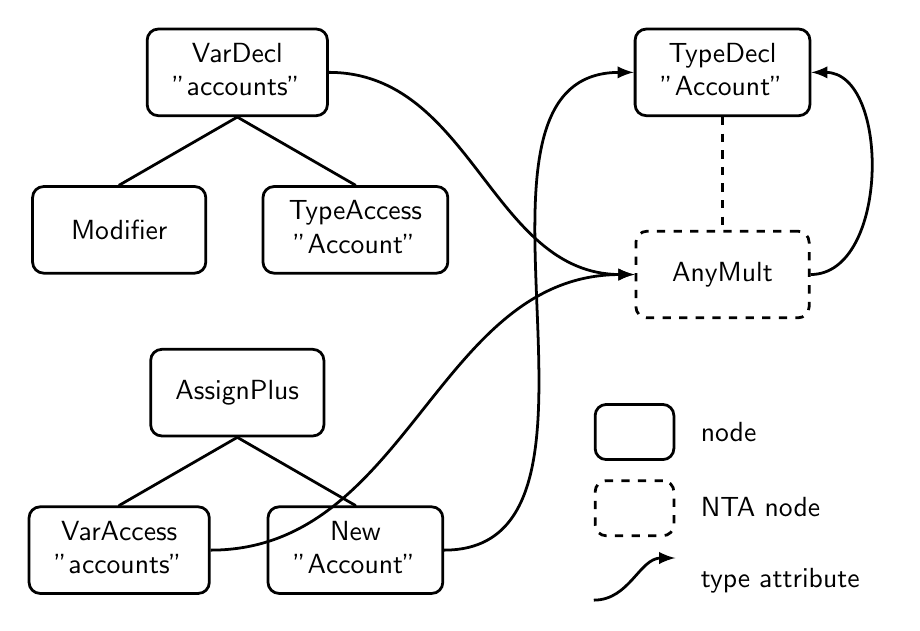
\begin{tikzpicture}[
    ast/.style={
      draw,
      line width=1pt,
      rounded corners,
      minimum width=2.2cm,
      minimum height=1.1cm
    },
    miniast/.style={
      ast,
      minimum width=1cm,
      minimum height=0.7cm
    },
    reference/.style={
      line width=1pt,
      -latex
    },
    edge from parent/.style={
      draw,
      line width=1pt,
      line cap=round,
      edge from parent path={(\tikzparentnode.south) -- (\tikzchildnode.north)}
    },
    level 1/.style={
      sibling distance=3cm,
      level distance=2cm
    }
  ]
  \node[ast] (decl) {\sffamily\begin{tabular}{cc}VarDecl\\"accounts"\end{tabular}}
    child { node[ast] (mod) {\sffamily{Modifier}} }
    child { node[ast] (type) {\sffamily\begin{tabular}{cc}TypeAccess\\"Account"\end{tabular}} }
  ;
  \node[ast,yshift=-3.5cm] (assign) at(decl.south) {\sffamily{AssignPlus}}
    child { node[ast] (use) {\sffamily\begin{tabular}{cc}VarAccess\\"accounts"\end{tabular}} }
    child { node[ast] (new) {\sffamily\begin{tabular}{cc}New\\"Account"\end{tabular}} }
  ;
  \node[ast,xshift=5cm] (typedecl) at(decl.east) {\sffamily\begin{tabular}{cc}TypeDecl\\"Account"\end{tabular}} ;
  \node[ast,dashed,yshift=-2cm] (any) at(typedecl.south) {\sffamily{AnyMult}} ;
  \draw[reference] (decl) to[out=0,in=180,looseness=1] (any);
  \draw[reference] (use)  to[out=0,in=180,looseness=1] (any);
  \draw[reference] (new)  to[out=0,in=180,looseness=1] (typedecl);
  \draw[reference] (any)  to[out=0,in=0,looseness=1] (typedecl);
  \draw[reference,dashed,-] (typedecl) -- (any);
  \node[miniast,yshift=-2cm] (astnode) at(any.west) {} ;
  \node[miniast,dashed,yshift=-0.6cm] (nta) at(astnode.south) {} ;
  \coordinate[yshift=-0.8cm] (a1) at(nta.south west);
  \coordinate[yshift=-1cm] (a2) at(nta.north east);
  \draw[reference] (a1) to[out=0,in=180,looseness=1] (a2);
  \node[anchor=west,xshift=2mm] (t1) at(astnode.east) {\textsf{node}};
  \node[anchor=west,yshift=-7mm] (t2) at(t1.south west) {\textsf{NTA node}};
  \node[anchor=west,yshift=-7mm] at(t2.south west) {\textsf{type attribute}};
  \end{tikzpicture}
  }%resizebox
\end{CenteredBox}
  \caption{AST with reference attributes (see text)}
  \label{figure6}
\end{figure}

\paragraph{Member Access} Multiplicities affect the analysis of member accesses
(qualified expressions). In regular Java code, the type of any qualified
expression is the type of the object on the right-hand side of the rightmost
dot. The qualifiers are only used for looking up the declaration of the
rightmost part. However, with multiplicities it is not sufficient to only
look at the multiplicity of the rightmost part -- the qualifying expression
multiplicities may affect the multiplicity of the whole expression. For
example, as discussed in \autoref{section3.4}, if the \inline{Account} class has a field
\inline{@option Bank bank}, the expression \inline{accounts.bank} will have the
multiplicity \emph{any}, although \inline{bank} has the multiplicity \emph{option}. This
is handled by extending the type analysis with attributes to find the
multiplicity of the left-hand part of a dot expression. The multiplicity of the
entire dot expression is computed using both the multiplicity of the left and
right parts, following \autoref{table1}.

\paragraph{Code Generation} The code generation constitutes the bulk of the
multiplicities implementation, translating from the higher-level operations on
multitudes to corresponding lower-level \inline{for}-loops, and handling all
the different combinations of multiplicities in assignments and expressions.
The implementation largely follows the translation scheme to a
multiplicity-free program proposed in \cite{ref37}; it is not repeated here for
space reasons (\autoref{section4} provided an outline, however).

\paragraph{Copying Hidden Collections} In the bytecode, multiplicity \emph{any}
is represented by a collection object (the hidden
collection), and care must be taken to not create aliases of these objects when
multiplicity values are copied. For this reason, we create a copy of the
collection object

\begin{itemize}
  \item when passing an \emph{any} as an argument to a method or
    constructor,
  \item when returning an \emph{any} from a method,
  \item at an explicit \inline{(@any)} cast, and
  \item when the multiplicity wrap expression either wraps or unwraps an
    \emph{any}.
\end{itemize}

\noindent The assignment to an \emph{any} does not need to
create a copy of the hidden collection of the right-hand side --- instead, the
objects of this collection are added to the cleared hidden collection of
the left-hand side.

Copying of collections can in many cases be avoided through static analysis and/or lazy
copying: In certain cases, we can deduce statically that the original
collection cannot be used anymore, for instance when returning the value of
a local variable. In these cases, copying is not needed. Another
optimization strategy is to represent a multitude by a wrapper object that
contains an internal collection. Copying can then be implemented lazily by
doing a shallow copy of the wrapper object, delaying the copying of the
internal object until it is modified. By letting the wrapper keep a
reference count, copying of the internal collection can be avoided for
wrappers whose internal collection is not shared by other wrappers.
We implemented such lazy collections as a library that we then benchmarked
against the regular, non-lazy collections in our case study (see
\autoref{section6.3} for the performance discussion).

\section{Case Study}
\label{section6}

\noindent To assess the impact of using multiplicities in a representative
case study, we looked for a subject program

\begin{enumerate}
  \item that uses a wide array of accepted object-oriented coding idioms so
    that multiplicities can be evaluated in a spectrum of constructions
    typically encountered in object-oriented programming,
  \item that is tightly covered by test cases so that accidental changes of
    functional behaviour induced by the use of multiplicities would quickly be
    discovered, and
  \item that can be run using file-based input that is openly available for
    reproduction of our performance observations (replication).
\end{enumerate}

\noindent Given these criteria, we selected the widely known regression
testing framework JUnit 4.0

\begin{enumerate}
  \item since it is renowned for its consistent use of design patterns and,
    generally, for its exemplary object-oriented style,
  \item since its own test suite is comprehensive, and
  \item since open-source programs are available whose test suites execute it,
    giving us the standardized program runs we wanted.
\end{enumerate}

\noindent Note in particular that every JUnit test suite tests not only the
program under test, but also JUnit itself against the suite's oracle: all
and only the tests of a program that pass using the original version of
JUnit should also pass using our modified version using multiplicities. We
selected JUnit 4.0 rather than one of its successors since it is manageable
in size and since it contains fewer features that are not used by the
majority of available JUnit test suites.

To manually obtain a version of JUnit that utilizes multiplicities in a
way that is both reproducible and that we deem to be representative of how
multiplicities will be used in practice, we changed the multiplicity of
every field having a collection type whose element type (type parameter) is
not a value type to \inline{@any} (and removed the collection type from the
type declaration), and every other field not having a value type to
\inline{@option}. We then changed the multiplicity of every other variable and
method return as required by the assignment compatibility and overriding
rules of multiplicities (see \autoref{section4.6}), unless where use of APIs (method
invocation and subclassing) required \emph{bare} parameters (in which
case a cast to \emph{bare} was introduced). The results of this
procedure are summarized in \autoref{table2}.

\begin{table}[h]
  \vspace{1em}
  \centering
  \begin{threeparttable}
    \begin{tabular}{l|ccc|c|c}
      \toprule
      & \emph{any} & \emph{option} & \emph{bare} & total & value-typed$^\dagger$ \\
      \hline
      fields & 11 & 44 & 121 & 176 & 29 \\
      returns & 9 & 34 & 249 & 292 & 108 \\
      formals & 3 & 83 & 642 & 728 & 403 \\
      locals & 7 & 34 & 482 & 523 & 380 \\
      casts to & 2$^\S$ & 21$^\$$ & 92 & 115 & \\
      \hline
      total & 32 & 216 & 1586 & 1834 & 920 \\
    \end{tabular}
    \begin{tablenotes}
      \small
      \item $^\dagger$ included in \emph{bare}
      \item $^\S$ implicit upcasts
      \item $^\$$ all downcasts from \emph{any}
    \end{tablenotes}
  \end{threeparttable}
  \caption{Multiplicities in declarations and casts}
  \label{table2}
\end{table}

\subsection{How Introduction of \texttt{@any} Changes Program Source}
\label{section6.1}

\noindent There were 11 collection-typed fields whose type parameter
(element type) was not a value type (cf.~\autoref{section3.6}), and which we changed
to multiplicity \emph{any}. Of these, 5 were originally declared \inline{final};
in 4 of these cases, the \inline{final} modifier had to be dropped since the
multitudes were actually modified after initialization (cf.~\autoref{section2.7}).
Introducing the multiplicity \inline{@any} (and changing the types;
cf.~\autoref{section3.2}) for these 11 fields required the subsequent change of 3 formal
parameters (one of which involved the removal of a wildcard; cf.~\autoref{section2.3}),
of 9 method returns, and of 7 local variables (giving us a total of 30
introduced \inline{@any} annotations; see \autoref{table2}). Of the remaining 27 uses
of collections, 9 were required by APIs, 5 held instances of value types, 3
were required by concurrent modification (iter/remove; see \autoref{section6.1.2}),
and the rest was used by local variables that never got a field assigned to
it (they could also have been changed to multiplicity \emph{any}).

Together with the introduction of \inline{@any} annotations, we replaced 12
invocations of \inline{add($\something$)} and 1 of \inline{addAll($\something$)} with \inline{+=}, and 2
invocations of \inline{remove($\something$)} with \inline{-=}; at the same time,
10 invocations of \inline{size()} where replace with \inline{|[$\something$]|} and 5
invocations of \inline{isEmpty()} were replaced with a test for null
(cf.~\autoref{section3.2}). There were 27 indexed accesses to list elements (using
\inline{get($\something$)}) in the original program where the list was replaced by an
\emph{any} multitude; all but 5 of these could be removed using
multiplicity downcasting (see \autoref{section6.1.3}); the remaining 5 required
wrapping (see \autoref{section6.1.2}).


\subsubsection{Loop Elimination}
\label{section6.1.1}

\noindent One of the supposed benefits of introducing \emph{any}
multiplicity is the elimination of loops (see Sections \ref{section2.1} and \ref{section3.4}).  And
indeed, 5 \inline{for}-loops over the elements of collections could be
replaced by plain member access on a corresponding multitude of objects. For
instance, we replaced the loop

\begin{lstlisting}
for (Runner each : fRunners)
  each.run(notifier);
\end{lstlisting}

\noindent (from \inline{CompositeRunner.run(RunNotifier)}) with

\begin{lstlisting}
fRunners.run(notifier);
\end{lstlisting}

\noindent In addition, even where the iteration variable is not used as the
left-most receiver in the loop expression (as above), it may still be
possible to eliminate the loop. For instance,

\begin{lstlisting}
for (Runner runner : fRunners)
  spec.addChild(runner.getDescription());
\end{lstlisting}

\noindent (from \inline{CompositeRunner.getDescription()}) was rewritten to

\begin{lstlisting}
spec.addChild(fRunners.getDescription());
\end{lstlisting}

\noindent after the multiplicity of the formal parameter \inline{description}
in

\begin{lstlisting}
public void addChild(Description description) {
  fChildren += description;
}
\end{lstlisting}

\noindent had been changed to \inline{@any} (note how this does not affect the
implementation of \inline{addChild($\something$)}).\footnote{In fact, increasing parameter multiplicity of \inline{add...(@option)} methods like the above allowed us to drop two \inline{addAll...(@any)} methods from the JUnit 4.0 source (they are now subsumed by the \inline{add...(@any)} methods).} However, because \emph{bare}
members may not be accessed on \emph{option} or \emph{any}
receivers (\autoref{section4.6}), this required the declaration of \inline{@option} as
the returned multiplicity of \inline{getDescription($\something$)} which, since
\emph{option} is not assignment compatible with \emph{bare}
(\autoref{section4.1}), required the subsequent introduction of 32 more
\inline{@option} annotations throughout the program. Yet, given that
\inline{@any} and \inline{@option} annotations are designed to be used together,
this does not appear to be counterproductive.

With a little redesign of programs, loop elimination can be pushed even
further. For instance, we found (in method \inline{createTest($\something$)} from class
\inline{JUnit4TestAdapterCache}) the loop

\begin{lstlisting}
for (Description child : description.getChildren())
  suite.addTest(asTest(child));
\end{lstlisting}

\noindent Here, the loop variable \inline{child} is the argument of another
method so that introducing multiplicity \inline{@any} for the parameter of
\inline{addTest($\something$)} as above is not sufficient --- \inline{asTest($\something$)} would need
to be changed to accept and return \emph{any} multiplicity as well,
which would require a major reworking of its implementation. However, as it
turned out, \inline{asTest($\something$)} can straightforwardly be moved to class
\inline{Description} (the class of its formal parameter, using the refactoring
Move Method \cite{ref16}), so that the loop can be replaced by

\begin{lstlisting}
suite.addTest(description.getChildren().asTest(this));
\end{lstlisting}

\noindent which is not only more succinct, but also more fluent\footnote{``fluent'' in the sense of a ``fluent API'':\\see \url{http://www.martinfowler.com/bliki/FluentInterface.html}} than the
original phrasing. In fact, this minor refactoring even allowed us to remove
a loop that was designed to fill a collection: we turned

\vbox{
\begin{lstlisting}
List<Test> returnThis = new ArrayList<Test>();
for (Description child : description.getChildren())
  returnThis.add(child.asTest(this));
return returnThis;
\end{lstlisting}
}

\noindent (from \inline{JUnit4TestAdapterCache.asTestList($\something$)}) into

\vbox{
\begin{lstlisting}
return new ArrayList<Test>(
  [[description.getChildren().asTest(this)]]
);
\end{lstlisting}
}

\noindent in which the \emph{any} multitude returned by
\inline{asTest($\something$)} is wrapped in a collection (note that API calls explicitly
expect the collection here; hence the name of the method, ``asTestList''!).

Of the 11 loops on the elements from a multitude that could not be
removed, 2 contained accesses of value-typed members (methods for counting
the number of leaves in a composite structure; see \autoref{figure4} for how this can
be simplified using collections), 3 used explicit iterators for removing
elements from the originally underlying collection (cf.~\autoref{section6.1.2}), and
6 had complex loop bodies that would have required major refactorings to
cast them to member access on \emph{any} expressions.

\subsubsection{Wrapping and Unwrapping Multitudes}
\label{section6.1.2}

\noindent We required a total of 15 wrappings or unwrappings:

\begin{itemize}
  \item In 5 cases, wrapping a multitude in a list was necessary because
    indexed access to individual objects was required and the dynamic
    multiplicity was not known to be 0 or 1 (in which case a downcast to \emph{option}
    would have been sufficient; cf.~\autoref{section4.5}).
  \item In 3 cases, wrapping a multitude into and subsequently unwrapping it
    from a local list-typed variable was necessary because of \inline{iter.remove()}
    loops.
  \item The remaining 4 wrappings and unwrappings were due to API calls.
\end{itemize}


\subsubsection{Multiplicity Casting}
\label{section6.1.3}

\noindent In Java without multiplicities, a multiplicity upcast (from
\emph{option} to \emph{any}) requires the wrapping of a single
object in a collection. For instance, the method whose header is declared as

\begin{lstlisting}
List<Throwable> getCauses(Throwable cause)
\end{lstlisting}

\noindent (from class \inline{ErrorReportingRequest}) returns the expression
\inline{Arrays.as}\inline{List(cause)} as a special case. In case \inline{cause} was
null, it would need to return an empty list, involving yet another clumsy
construction (see \autoref{section6.1.5}). Using multiplicities, the same method is
declared as

\begin{lstlisting}
@any(List) Throwable getCauses(@option Throwable cause)
\end{lstlisting}

\noindent for which \inline{cause} is a type-correct and multiplicity-correct
return expression (the multiplicity upcast is implicit here).

Multiplicity downcasts (from \emph{any} to \emph{option}) are
somewhat more involved. In standard Java, this would require the test of the
size of a collection and, in case it is 1, the extraction of the sole
element of the collection (the cast would result in \inline{null} if size is
0, or else raise an exception). Indeed, we found 24 of constructions such as

\begin{lstlisting}
Failure failure= result.getFailures().get(0);
assertEquals(expected, failure.getDescription());
\end{lstlisting}

\noindent in JUnit, which silently assumes that there is at least one
failure and ignores possible failures beyond the first (actually, it leaves
unstated whether there may be additional failures). Using multiplicities, we
can rewrite the first line to

\begin{lstlisting}
@option Failure failure= (@option) result.getFailures();
\end{lstlisting}

\noindent which makes the cast explicit and states that there should be at
most one failure (which proved to be the correct assumption in 17 out of the
24 occurrences of this pattern).

\subsubsection{Enforce Proper Encapsulation of Multitudes}
\label{section6.1.4}

\noindent As noted in \autoref{section2.4}, fields holding collections should be
encapsulated and not be passed to clients via getters. Nevertheless, we find
in JUnit's class \inline{Description} the method

\begin{lstlisting}
public ArrayList<Description> getChildren() {
  return fChildren;
}
\end{lstlisting}

\noindent allowing clients to bypass the public method \inline{addChild($\something$)}
supplied by the same class for directly manipulating the children of
\inline{Description} objects. After replacing the declaration of the field
\inline{fChildren} in \inline{Description} with

\begin{lstlisting}
@any(ArrayList) Description fChildren;
\end{lstlisting}

\noindent and adjusting the above declaration of \inline{getChildren()}
accordingly, an invocation of
\inline{get}\inline{Children().add($\something$)} will have no effect
on \inline{fChildren}, since \inline{getChildren()} no longer returns an alias
of it (\autoref{section3.5}). As it turns out, however, the sole occurrence of a
manipulation of \inline{fChildren} in JUnit via \inline{getChildren()} is in the
body of \inline{addChild($\something$)} itself:

\begin{lstlisting}
public void addChild(Description description) {
  getChildren().add(description);
}
\end{lstlisting}

\noindent Here, the idea of Self Encapsulate Field \cite{ref16} clearly conflicts
with how collections should be encapsulated (see \autoref{section2.4}). Using
multiplicities, the body of \inline{addChild($\something$)} is rewritten to

\begin{lstlisting}
fChildren += description;
\end{lstlisting}

\noindent while that of \inline{getChildren()} can remain as is, without
granting true clients access to \inline{fChildren}.

While the use of multiplicities enforces proper encapsulation as shown
above, it can also help avoid explicit cloning, as found in class
\inline{TestResult}:

\begin{lstlisting}
synchronized List<TestListener> cloneListeners() {
  List<TestListener> result= new ArrayList<>();
  result.addAll(fListeners);
  return result;
}
\end{lstlisting}

\noindent Here, using multiplicity \emph{any} it suffices to return
\inline{fListeners} in the body of the method (which needs to remain
synchronized --- all multiplicity operations are non-synchronized by default).

\subsubsection{Uniform Use of \texttt{null}}
\label{section6.1.5}

\noindent The fact that relating to no object in a to-many relationship is commonly
represented by an empty collection (cf.~\autoref{section2.2}) has led to the
introduction of special collection classes (e.g.,
\inline{Collections.EmptyList}, \inline{Collections.EmptySet}, both from
\inline{java.util}) whose sole instances represent an empty collection. For
instance, the method declared as

\begin{lstlisting}
List<Throwable> validateAllMethods(Class<?> clazz)
\end{lstlisting}

\noindent (from class \inline{ParameterizedTestMethodTest}) returns
\inline{Collections.emptyList()} as a special case (an upcast from
multiplicity \emph{none} to \emph{any}). Replacing the declaration
of the method with

\begin{lstlisting}
@any(List) Throwable validateAllMethods(Class<?> clazz)
\end{lstlisting}

\noindent allows the method to return \inline{null} instead, which has the same
meaning as \inline{null} for \inline{@option}, i.e., is subsequently
interpreted as no object (and, unless it is cast to \inline{@bare}, cannot
cause a null pointer exception). Note that the fact that, unlike
\inline{Collections}\discretionary{}{}{}\inline{.emptyList()}, the returned multitude is mutable maintains
behavioural subtyping \cite{ref22}: while

\begin{lstlisting}
@any(List) Throwable result = null;
result += new Throwable("it's OK!");
\end{lstlisting}

\noindent is indeed OK, the seeming equivalent

\begin{lstlisting}
List<Throwable> result = Collections.emptyList();
result.add(new Throwable("not OK!!"));
\end{lstlisting}

\noindent causes an ``unsupported operation'' exception.

\subsubsection{Uniform Call Semantics}
\label{section6.1.6}

\noindent The fact that method calls are by value effectively (i.e., a
method cannot modify the multitude that it gets passed; cf.~\autoref{section3.5})
means that methods such as \inline{void Collections.sort(List<T>)} (which
would need to be rewritten to \inline{void} \inline{Collections}\discretionary{}{}{}\inline{.sort(@any(List) T)}) no
longer work, simply since sorting has no effect on the multitude that is
passed into the method. To fix this, we wrote our own sort method that
returns a sorted multitude which can be assigned back to the variable
holding the original multitude. Specifically, we changed 2 invocations of
the kind

\begin{lstlisting}
Collections.sort(fRunners, $\something$)
\end{lstlisting}

\noindent (here from class \inline{CompositeRunner}) to

\begin{lstlisting}
fRunners = Multiplicities.sort(fRunners, $\something$)
\end{lstlisting}

\noindent where \inline{Multiplicities} is a helper class analogous to
\inline{Collections}. Note how this makes clear why \inline{fRunners} cannot be
declared \inline{final}, since the multitude is in fact changed (even though
the collection secretly holding it has remained the same object; cf.~\autoref{section2.7}).

\subsection{How Introduction of \texttt{@option} Changes Program Source}
\label{section6.2}

\noindent Changing the remaining fields that did not have value types to
multiplicity \emph{option}, and subsequently also formal parameters,
method returns, and local variables as required by the rules of \autoref{section4.1},
gave us a total of 44 fields, 34 returns, 83 formal parameters, and 34
locals, all with multiplicity \emph{option} (see \autoref{table2}).

\subsubsection{Elimination of Tests for Not Null}
\label{section6.2.1}

\noindent Just like the use of \emph{any} can eliminate loops, the use
of \emph{option} can eliminate tests for not null (\autoref{section4.6}). As it
turns out, however, JUnit does not make much use of the value \inline{null}
representing ``no object'': in fact, in the whole of JUnit there is no
test for not null on a field that could be declared with \inline{@option}, and
only a single test for null (which is however only used for lazy
initialization of the field). However, there are some tests for not null on
local variables, one of which,

\begin{lstlisting}
Runner childRunner= Request.aClass(each).getRunner();
if (childRunner != null)
  runner.add(childRunner);
\end{lstlisting}

\noindent (from method \inline{ClassesRequest.getRunner()}), we could rewrite
to

\begin{lstlisting}
runner.add(Request.aClass(each).getRunner());
\end{lstlisting}

\noindent This was possible since method \inline{add($\something$)} accepts
\emph{any} multiplicity and \inline{getRunner()} returns
\emph{option} multiplicity, and since \inline{null} uniformly means
``no object'' for \emph{option} and \emph{any} multiplicities
(see Sections \ref{section3.2} and \ref{section4.6}).

\subsubsection{Multiplicity Casting}
\label{section6.2.2}

\noindent While explicit and implicit multiplicity casts to
\emph{option} and \emph{any} avoid clumsy coding idioms
(\autoref{section6.1.3}), the current well-formedness rules of multiplicities may also require
explicit downcasts to \emph{bare} (cf.~\autoref{section4.5}), which can be a
nuisance. Specifically, the fact that value-typed members (which must be
\emph{bare}) may not be accessed on receiver expressions with
multiplicity \emph{option} (Sections \ref{section3.6} and \ref{section4.6}) can require annoying
casts. For instance, in

\begin{lstlisting}
public int countTestCases() {
  return ((@bare) fRunner).testCount();
}
\end{lstlisting}

\noindent (from class \inline{JUnit4TestAdapter}) the cast \inline{(@bare)} is
required since \inline{fRunner} has multiplicity \emph{option} (meaning that
it may evaluate to no object) and \inline{testCount()} returns an integer.
Even though the cast \inline{(@bare)} can be read as a warning that a null
pointer exception may occur here (which can never occur when dereferencing
\emph{option} or \emph{any} receivers; see \autoref{section3.4}), given
that we needed to insert 62 such casts in JUnit (cf.~\autoref{table2}; the remaining
30 casts to \emph{bare} were needed for interfacing the JDK and
assertions), not all programmers will regard this aspect of our language
design as ideal. An elegant solution to this problem seems to be the
introduction of \emph{one} as an additional multiplicity annotation
(for relating to precisely 1 object) and to allow access of \emph{bare}
members on \emph{one} receivers with resulting multiplicity
\emph{bare}. However, since this would require our notion of
multiplicities to be integrated with existing not-null annotations and
checks, we have left this to future work (\autoref{section8.1}).

\subsection{Performance Observations}
\label{section6.3}

\noindent To check the correctness of our multiplicity compiler, we ran
JUnit's own test suite on our multiplicity-enhanced version of JUnit (named
``JUnit-M''), and also on the test suites of three additional
multiplicity-free benchmark programs listed in \autoref{table3}. All tests gave
the same results, suggesting that the modified and the original version of
JUnit are functionally equivalent. There were 25 test cases that failed in
both versions (for AC Lang), because they require a newer runtime version of
JUnit. We decided to keep these tests since they exercise failing behaviour
in JUnit. All other tests that could be compiled with JUnit 4.0
(cf.~\autoref{table3}) passed.

To check how multiplicities affected the execution time of JUnit-M, we
compared running the following different compiled versions of JUnit:

\begin{itemize}
  \item \emph{ju4jc}: original JUnit 4.0 compiled using javac from OpenJDK 7, i.e.,
    the reference compiler for Java.
  \item \emph{ju4jj}: original JUnit 4.0 compiled using JastAddJ for Java 7.
  \item \emph{ju4m}: JUnit-M 4.0 compiled with our multiplicity-enhanced compiler
  \item \emph{ju4l}: JUnit-M 4.0 compiled with a variant of our multiplicity-enhanced
    compiler that uses lazy copying of collections, as described at the end of
    \autoref{section5}.
\end{itemize}

\noindent We used these four different versions of compiled JUnit to run the
test suites in \autoref{table3}, all of which were compiled using javac.

\begin{table}[h]
  \vspace{1em}
  \begin{center}
  \begin{threeparttable}
    \begin{tabular*}{0.75\textwidth}{l|c @{\extracolsep{\fill}}}
      \toprule
      \emph{Subject program and Version} & \emph{Number of Test Cases} \\
      \hline
      Apache Commons Codec 1.3 & 191 \\
      Apache Commons Lang 3.0 & 1923$^{\dagger\S}$ \\
      Jaxen 1.1.6 & 716$^\$$ \\
      JUnit 4.0 & 255 \\
    \end{tabular*}
    \begin{tablenotes}
    \small
    \item $^\dagger$ excluding 10 that we had to remove because they could not be compiled with JUnit 4.0
    \item $^\S$ 25 of these tests fail both with and without multiplicities because they should normally be run with JUnit 4.7 (see text)
    \item $^\$$ excluding 2 that were removed because they contain an infinite loop (see text)
    \end{tablenotes}
  \end{threeparttable}
  \end{center}
  \vspace{-1em}
\caption{Subject programs used in the evaluation.}
\label{table3}
\end{table}

\paragraph{Steady-state performance} We measured execution time in steady state, i.e.,
after running for a while so that the optimizing JIT compiler has
\emph{warmed up}, and reached a stable state. This is a relevant test
scenario for long running applications. However, to use this method on the
JUnit test suite, we had to remove two test cases that include an infinite
loop that can be stopped only by a call to \inline{System.exit()}
(thereby terminating the host JVM).

To measure on steady state, we used the \emph{multi-iteration determinism}
method for benchmarking from Blackburn et al. \cite{ref5}, which
includes the following steps:

\begin{enumerate}
  \item The benchmark is iterated $N-1$ times in the same JVM to achieve steady-
    state for the JIT.
  \item JIT optimization is then turned off to not further affect the
    measurements.
  \item One more iteration of the benchmark is made, but is not measured.
  \item Finally, $K$ iterations are made, measuring the execution time of each.
\end{enumerate}

\noindent During different runs (consisting of $N+K$ iterations of the
benchmark), the JIT may stabilize on different states, due to the
non-determinism of the JIT optimization. For this reason, we make $R$ runs
for each benchmark, and compute the arithmetic mean of the means of the $K$
iterations in each run, and the 95\% confidence interval, as suggested by
Georges et al \cite{ref17}. For our measurements we chose $R=15$, $N=30$, and
$K=20$. \autoref{table4} shows the results of our steady-state experiments.

\begin{table}[h]
  \vspace{1em}
  \centering
\begin{tabular}{l|ccccc}
  \toprule
  & ju4jc & ju4jj & ju4m & ju4l & ju4m/ju4jj loss \\
  \hline
  \emph{AC Codec} & & & & & \\
  mean & 172 & 169 & 178 & 204 & 0.0530 \\
  conf. int. & $\pm16.5$ & $\pm15.2$ & $\pm15.5$ & $\pm2.7$ & \\
  \hline
  \emph{AC Lang} & & & & & \\
  mean & 6747 & 6748 & 6750 & 6758 & 0.0003 \\
  conf. int. & $\pm2.6$ & $\pm2.6$ & $\pm2.2$ & $\pm2.3$ & \\
  \hline
  \emph{Jaxen} & & & & & \\
  mean & 249 & 248 & 249 & 258 & 0.0033 \\
  conf. int. & $\pm3.1$ & $\pm1.0$ & $\pm1.3$ & $\pm1.3$ & \\
  \hline
  \emph{JUnit} & & & & & \\
  mean & 845 & 848 & 853 & 867 & 0.0053 \\
  conf. int. & $\pm2.2$ & $\pm2.3$ & $\pm2.6$ & $\pm3.1$ & \\
\end{tabular}
\caption{Execution times (in msecs).}
\label{table4}
\end{table}

In comparing \emph{ju4jj} and \emph{ju4m}, we anticipated there
to be a performance loss due to copied collections and extra null checks. We
can see that there is a tendency to a slight performance loss when using
multiplicities for all four benchmarks. However, the confidence intervals
overlap, and the difference between the means is only 5\% for AC Codec, and
less than 1\% for the other benchmarks. We therefore regard the performance
loss as negligible. We can also note that the performance of the javac
compiler and the JastAddJ compiler (\emph{ju4jc} and \emph{ju4jj})
are almost the same, indicating that the results should transfer to javac,
should one wish to implement multiplicities there.

\paragraph{Using Lazy Copying} \autoref{table4} also shows the results from running
\emph{ju4l}, i.e., JUnit-M compiled with a variant of our
multiplicity-enhanced compiler that implements lazy copying of collections,
as discussed at the end of \autoref{section5}. Unfortunately, the results show that
the use of lazy copying degrades the performance, rather than improving it.
We measured the number of copied collections (\autoref{table5}) and their sizes, and
found that around half of the collections had size 0 and that less than 1\%
had a size larger than 10. Apparently, because the collections are so small,
the cost of copying the hidden collection is lower than the cost of delegating all method calls through an intermediate lazy collection.
Further investigation is
needed to see if the implementation of the lazy copying can be improved, and
if it can be useful for other benchmarks.

\begin{table}[h]
  \vspace{1em}
  \centering
\begin{tabular}{l|ccccc}
  \toprule
  & \emph{AC Codec} & \emph{AC Lang} & \emph{Jaxen} & \emph{JUnit} \\
  \hline
  collection copies & 1007 & 20326 & 8038 & 8105 \\
  avoided using lazy & 778 & 16516 & 6554 & 6884 \\
  checking not null & 1045 & 8417 & 3112 & 3310 \\
\end{tabular}
\caption{Instruction overhead}
\label{table5}
\end{table}

\subsection{Discussion}
\label{section6.4}

\noindent As the examples of \autoref{figure3} and \autoref{figure4} suggest, savings in terms
of the number of tokens used in a program fragment can be considerable.
Also, \autoref{section6.1.1} presented several interesting examples of loop
elimination enabled by member access on multitudes of objects. In a complete
program, however, savings are diluted, and the total number of tokens can
even increase because of the additional annotations required in
declarations. In fact, in our case study the multiplicity-enhanced version
has 151 more tokens than its original. However, this increase is explained
by the additional annotations used in declarations, whereas the number of
tokens in the other statements (instructions) are reduced. The possible
reduction of tokens in the instructions is currently diminished by the casts
to \emph{bare} that we had to introduce for interfacing with API code
and accessing \emph{bare} members (\autoref{section6.2.2}). We expect these
numbers to improve with the introduction of \emph{one} as an additional
multiplicity, and of course with the migration of APIs.

\section{Related Work}
\label{section7}

\noindent Smalltalk not only comes with a powerful collections library, with
its indexed instance variables it also offers a way of directly associating
one object with a multitude of other objects, without reifying this
association \cite{ref19}. However, since indexed integer variables are unnamed (they
are similar to the so-called indexers of the .NET languages \cite{ref23}), there can
be only one set of indexed instance variables per object, limiting their use
for implementing relationships (of which an object may have many). And yet,
indexed instance variables share with our \emph{any} fields that two objects
cannot share the same set of indexed instance variables (i.e., there is no
aliasing of multitudes).

The object constraint language (OCL) \cite{ref6, ref27}, which is used to express
conditions of well-formedness of UML models, allows the dereferencing
(``navigation'') of attributes and associations with arbitrary multiplicities
using the dot notation. However, OCL still reifies multitudes of objects
using collections; the difference between one and many objects (singular and
plural) is mitigated only slightly by allowing collection operations to be
applied to single objects also. This is different for Alloy \cite{ref21}, a textual
modelling language which maps object-orientation to relational logic and in
which the notion of multiplicity is also prominent. Unlike OCL, Alloy does
not distinguish between scalars and sets, and treats scalars as singletons.
This largely removes the differences between one and many objects from Alloy
expressions (which we strive for also); however, like OCL, Alloy is not a
programming language.

The programming languages JavaFX\texttrademark{} \cite{ref38} and C$\omega$ \cite{ref2} offer sequences,
or streams, as array-like type constructors for variables with multiplicities
greater than 1. Like arrays, sequences are reified multitudes of objects;
however, unlike arrays, they are immutable and have value semantics.
Sequences cannot be nested --- any attempt to do so results in a flat
sequence. \inline{null} in the context of a sequence means the empty
sequence and a scalar value means a singleton sequence, so that both can be
assigned to a sequence-typed variable. In C$\omega$, a stream can occur as the
receiver of a member access; this access is then mapped over the elements of
the stream, yielding a stream of the member type (so that chained member
accesses on streams are possible). While this generalized member access has
the same semantics as corresponding expressions in OCL and Alloy, the
suitability of streams (which have been subsumed by iterators in C\# 3.0 \cite{ref4})
for implementing relationships to many objects is limited by their
immutability.

The semantics of our static multiplicity \emph{option} is somewhat
similar to using the \inline{Option} class in Scala \cite{ref29}: a receiver of type
\inline{Option} can be \inline{None}, in which case applying a function (using
\inline{map} or \inline{flatMap}) produces \inline{None}. Similarly, a function
can be applied to a collection (again using \inline{map} or \inline{flatMap}),
resulting in a collection of the same type, containing the return values.
The main difference to object-oriented programming with multiplicities as
put forward here is that we use no container types, but instead separate
type from multiplicity, avoiding the awkward dominance of the container type
over the content type \cite{ref37} imposed by wrappers such as \inline{Option} and
collections. Another difference is that in object-oriented programming with
multiplicities as we implemented it, the use of \inline{flatMap} to apply
functions to \emph{option} and \emph{any} multiplicities is implicit.

Ungar and Adams have recently presented a parallel programming language Ly
that offers so-called \emph{ensembles} as an alternative to collections
\cite{ref39}. Ensembles accommodate member objects that, when the ensemble is sent a
message, all respond in parallel. However, unlike our multitudes of objects,
an ensemble in Ly is a first-class object, and a singleton ensemble is
different from the object that it contains. Since Ly is untyped, runtime
checks are required to avoid that an ensemble contains itself (which may
lead to infinite recursion when a message received by an ensemble is
forwarded to itself). Also, empty ensembles are currently not integrated
seamlessly, and demand further dynamic checks. It seems that the
multiplicities described in this paper would solve at least some of the
problems incurred by ensembles (but notably not those related to
parallelism).

While implementing relationships to many objects using collections (or
similar reifications of multitudes) is by far the most commonly used pattern
\cite{ref26}, automatic mappings from object-oriented models to programs may
introduce other, more sophisticated patterns \cite{ref18}. Both are however
challenged by integrating relationships in object-oriented programming as a
native concept.

As far back as 25 years ago, Rumbaugh argued for the lifting of the
field-and-collection based relationship encodings of object-oriented
programs to the level of a first class language construct \cite{ref34}. For this
purpose he introduced relations as instances of a special class
\inline{Relation} that has fields holding a relation declaration (i.e., the
types of the participants, role names, cardinalities, etc.), as well as a
field holding the extension of the relation (i.e., its tuples). Unlike in
many other approaches that followed, an instance of \inline{Relation}
represents a relation, not a tuple; standard operations Rumbaugh defined on
these instances included the adding and removal of tuples, indexed access to
tuples of the relation, and scanning of the relation (iterating over its
tuples). Later, Rumbaugh also added propagation attributes to relations
which allowed the controlled recursive propagation of certain method
invocations through object graphs \cite{ref35}; however, this is not to be confused
with our lifting of method invocations from single objects to multitudes of
objects. While Rumbaugh's proposals amount to embedding a native
implementation of (parts of) a relational database system in
object-oriented programs, our approach of implementing to-many references is
lightweight. Also, our relationships (represented by multitudes of objects)
are not first-class.

\O{}sterbye picked up Rumbaugh's proposals and presented a Smalltalk-based
association compiler that can choose between internal and external
implementations of relationships \cite{ref32}. An internal implementation keeps the
information which other objects an object is related to local to the object,
whereas an external implementation uses first class relationship objects for
this purpose. Independent of the implementation choice, \O{}sterbye, like
Rumbaugh before him, offers role-based and association-based access to
relationships. However, in his role-based access protocol, he distinguishes
between to-one and to-many relationships, continuing the discontinuity we
want to rid programming of. This discontinuity is preserved in \O{}sterbye's
subsequent work \cite{ref31}, in which he leaves the untyped realm of Smalltalk
to present a library-based approach for C\#. In his library, association
classes are complemented by role classes providing for internal
implementation of relationships. However, given the fundamental meaning
relationships have in most problem domains, we argue for a native, rather
than a library-based, integration of relationships.

Bierman and Wren's RelJ is based on a formalized notion of relationships
as first class types whose instances, called relationship instances, are
tuples \cite{ref3}. These tuples, which --- like objects --- can have state
and behaviour, are created and returned by adding a pair of objects to a
relationship. Navigation of a relationship always results in a set having
value semantics, making the result of navigation covariant with the target
type of the navigation \cite{ref3}. However, sets cannot be the source of
navigation, so that navigation cannot be chained as in our approach. Bierman
and Wren also suggest how multiplicities can be restricted statically, using
\emph{one} (for $[0,1]$, analogous to our \emph{option}) and \emph{many}
(for $[0,*]$, analogous to our \emph{any}) annotations; the invariant imposed
by \emph{one} is then enforced by changing the semantics of adding to a
relationship with that of replacing an instance of a relationship
(destructive update, or assignment). By contrast, we have restricted the
additive update (\inline{+=}) to \emph{any} multiplicities, and require a
downcast from \emph{any} to \emph{option} for an assignment to
\emph{option}, protecting us from a silent change of behaviour when a
multiplicity is changed from \emph{any} to \emph{option}.

The relationship aspects of Pearce and Noble use the intertype
declarations of AspectJ to shift the bookkeeping necessary for maintaining
relationships between objects from the objects to relationships \cite{ref33}. The
relationships are coded as aspects which can carry additional,
relationship-specific behaviour. Class definitions remain ignorant of the
relationships for which they supply the participants, which is considered an
increase in the separation of concerns. This separation goes too far,
however, when an object needs access to others it is related to --- in that
case, it has to query the relationship it was to be kept unaware of.

In the language Rumer, references to objects are completely expelled from
so-called entity types (conventional classes), and objects are related
exclusively through relationship types \cite{ref1}. It follows that, analogous to
the relationship aspects of Pearce and Noble \cite{ref33}, only relationships know
which entities are related (referred to as stratification in \cite{ref1}). Entity
and relationship types have associated extent types which are instantiated
and populated explicitly by the programmer. Relationships can be nested, and
relationship extents can be owned by relationships, so that they cannot
escape the owning relationship. While owned relationship extents bear some
resemblance to our multiplicities (which likewise cannot be aliased), the
whole approach seems rather heavy weight --- in particular, with all knowledge
about relationships fully encapsulated in relationships (so that objects are
ignorant of whether and how they are related), much of an application's
logic (including that captured in most methods) has to be moved to
relationships, with objects being degraded mostly to passive data containers
with identity. This means a fundamental paradigm shift for object-oriented
programming, and migrating an existing application to the concepts embodied
in Rumer will amount to a major redesign effort.

\section{Future Work}
\label{section8}

\subsection{Integrating NonNull}
\label{section8.1}

\noindent As noted in \autoref{section6.2.2}, introduction of multiplicity
\emph{one} would help avoid an unpleasant restriction concerning the
access of \emph{bare} members via \emph{option} receivers. The
multiplicity \emph{one} is equivalent to annotating a type use as being
\emph{NonNull} like in, for example, the Checker framework \cite{ref11}.
Additionally, \inline{(@one)} can be used as a cast on an expression.
Fähndrich and Leino showed how \emph{NonNull} can be implemented to
handle initialization correctly, introducing the notion of raw types \cite{ref15}.
This solution has been implemented for a previous version of JastAddJ \cite{ref14}.
A natural next step for us is thus to extend our implementation of
multiplicities with this solution, supporting multiplicity \emph{one}.
We expect this to allow us to replace the multiplicity of most
\emph{bare} variables with \emph{one}, and hence to reduce the
number of casts substantially, as \emph{one} expressions can safely be
used as arguments to library methods requiring bares, and \emph{bare}
members (value types!) can safely be accessed on \emph{one} receivers.
Additionally, by adding type annotations, as introduced in Java 8,
\inline{@NonNull} annotations can be represented by \emph{one}
multiplicities, and be typechecked by the compiler.

\subsection{Qualified Access}
\label{section8.2}

\noindent As noted in \autoref{section4.1}, a collection \inline{C} used in an
\inline{@any(C)} annotation must have a single type parameter representing
the type of the elements of the collection. This requirement excludes maps
from a key type to a value type (such as \inline{HashMap<K, V>}). Not
excluded, but not especially supported are indexed collections (like
\inline{ArrayList}\inline{<E>}), which are special maps (with positive integers as
keys): read access of the $i^{th}$ object to which an expression \inline{e} with
multiplicity \emph{any(List)} evaluates currently requires
the clumsy workaround \inline{[[e]].get(i)}; write access is even clumsier
(not shown here). For qualified access of the objects among a multitude,
lists and maps can be generalized to associative arrays, effectively
implementing the qualified associations of UML \cite{ref28}. However, we have not
yet investigated the language extensions this would require.

\subsection{Case Studies on Modelling and Grammar Frameworks}
\label{section8.3}

\noindent Our current case study focuses on making use of multiplicities for
ordinary Java code. Another interesting focus for case studies would be to
focus on modelling frameworks such as EMF, where an API is generated from a
metamodel expressing relations with cardinalities. It would be interesting
to investigate how multiplicities could be used to simplify both the API and
its usage. Furthermore, an interesting avenue of research would be to
investigate to what extent metamodels can be automatically computed from
code using multiplicities, reducing the gap between models and code.

In a similar manner, it would be interesting to investigate how
multiplicities can simplify abstract syntax tree APIs, as generated by many
compiler tools from EBNF-like formalisms. Here, there is a natural match
between the typical \emph{child}, \emph{optional} and
\emph{list} constructs and the \emph{one}, \emph{option} and
\emph{any} multiplicities.

\subsection{Refactoring to Multiplicities}
\label{section8.4}

\noindent In our experiment described in \autoref{section6} we refactored JUnit
manually from ordinary Java code to code using multiplicities. An
interesting opportunity for further research is to design automated
refactorings for this purpose. Based on the current case study we can see
that most of these refactoring cases are fairly simple (they are related to
a Change Declared Type refactoring), but also that there are a number of
challenges that need to be addressed to find a general refactoring approach.

\section{Conclusion}
\label{section9}

\noindent Letting expressions evaluate to any number of objects (rather than
just one), and handling multitudes of objects that are not reified as one
object, means a departure from object-oriented programming as we know it. In
this paper, we have picked up a proposal for implementing object-oriented
programming with multiplicities presented at last year's {Onward!} conference \cite{ref37},
and turned it into a fully functional compiler of Java 7 that can
handle multitudes of objects as proposed. We tested this compiler by
changing the source code of JUnit 4.0 so that it utilizes multiplicities,
and by using the binaries produced by the compiler in place of the original
binaries for running a number of different open source test suites on their
programs under test. Functionally, both binaries are equivalent;
furthermore, observed performance measures suggest that using multiplicities
in JUnit 4.0 imposes only minor penalties. At the same time, a detailed
analysis of the changes performed on the JUnit sources suggests that
programs can indeed be simplified using multiplicities, avoiding many of the
peculiarities imposed by using collections as containers of multitudes.

% bibtex
%\bibliographystyle{alphaurl}
%\bibliography{jot2014}{}

\section*{Acknowledgments}

This work was in part financed by the Swedish Research Council under grant 621-2012-4727.

% biblatex
{\raggedright
\printbibliography[segment=\therefsegment,heading=subbibliography]
}

}
